% Author: Zhehao Wang 404380075 zhehao@cs.ucla.edu

% Thanks to Haitao Zhang for helping with (trying to) catch up with the class, and with the latex template
% Grammar package: http://tex.stackexchange.com/questions/24886/which-package-can-be-used-to-write-bnf-grammars

\documentclass{article}
\topmargin = 0in
\oddsidemargin = 0in
\evensidemargin = \oddsidemargin
\textwidth = 6.5in
\textheight = 8in
\usepackage{amsthm}
\usepackage{amsmath}
\usepackage{syntax}
\usepackage{graphicx}

\usepackage{algorithm}
\usepackage[noend]{algpseudocode}

\makeatletter
\def\BState{\State\hskip-\ALG@thistlm}
\makeatother

\title{CS180 Homework 2}
\author{Zhehao Wang 404380075 (Dis 1B)}
\date{Apr 10, 2016}

\begin{document}
\maketitle

\begin{description}

\item[1]{Number of inversions remains unchanged for any permutation}
  
  \textbf{Proof by induction on the number of pair swaps in the permutation:} we denote the original lists as $A = {a_1...a_n}$ and $B = {b_1...b_n}$. Each permutation consists of a number of pair swaps for songs in both list A and B. We call a pair $(a_i, a_j)$ \textit{flipped} if it used to be $(a_i, a_j)$ before the permutation, and becomes $(a_j, a_i)$ after the permutation, and the songs $a_i$, $a_j$ to be \textit{involved} in the flip.

  \textbf{Base case:} consider the case where only one pair in both A and B is swapped in the permutation. Denote the pair as $(a_i, a_j)$ in the original list A, where $i < j$. We can find the same songs in B where $a_i = b_m$ and $a_j = b_n$. The sequence in B could be $(b_m, b_n)$, or $(b_n, b_m)$. Consider the $(b_m, b_n)$ where $m < n$ case first:

  The \textit{flipped} pairs in A caused by this permutation include: $(a_i, a_j)$, $(a_p, a_j)$ and $(a_i, a_p)$, where $i < p < j$. Similarly, \textit{flipped} pair in B include: $(b_m, b_n)$, $(b_q, b_n)$ and $(b_m, b_q)$, where $m < q < n$. Since $a_i = b_m$ and $a_j = b_n$, number of inversions is not changed by A and B both having the $(a_i, a_j)$, $(b_m, b_n)$ flips. Thus we consider each $a_p$ and $b_q$ \textit{involved} in the flip, and the total number of inversions does not change if each \textit{involved} $a_p$ and $b_q$ do not cause changes in the total number of inversions. Case analysis on the position of each $b_l$ in B where each $b_l = a_p$.
  
  \begin{itemize}
  \item
  If $l < m$, then list B used to have $(b_l, b_m)$ and $(b_l, b_n)$, list A used to have $(a_i, a_p)$ and $(a_p, a_j)$, number of inversions used to be 1. After the permutation, B still has $(b_l, b_m)$ and $(b_l, b_n)$, and A has $(a_p, a_i)$, $(a_j, a_p)$. Number of inversions is still 1.

  \item
  If $l > n$, the case is similar with above. The number of inversions before and after the permutation are both 1.

  \item
  If $m < l < n$, then B used to have $(b_m, b_l)$ and $(b_l, b_n)$, A used to have $(a_i, a_p)$ and $(a_p, a_j)$, and number of inversions used to be 0. After the permutation, B has $(b_l, b_m)$ and $(b_n, b_l)$, A has $(a_p, a_i)$ and $(a_j, a_p)$. The number of inversions is still 0.
  \end{itemize}

  Similar case analysis can be done for each $a_k$ in list A where each $a_k = b_q$. We have the number of inversions does not change when B's sequence is $(b_m, b_n)$. 

  Similar case analysis can be done when B's sequence is $(b_n, b_m)$, with the only difference being that in case 3 ($n < l < m$), the number of inversions before and after the permutation are both 2 instead of 0. Thus to summarize, we have the number of inversions does not change when only one pair is swapped in the permutation.

  \textbf{Induction case:} assume that the conclusion holds for any permutation involving $n$ pair swaps. For any permutation involving $n+1$ pair swaps, by the induction hypothesis, we know that the conclusion holds for its sub-permutation with one pair excluded. By applying the analysis of the base case on the results of the sub-permutation, we know that the conclusion holds for any permutations involving $n+1$ pair swaps as well.
  

\item[2]{Number of intersection and inversions}

  (a)

  \textbf{Proof:} an inversion if defined by a pair $(i, j)$ such that $q_i$ is before $q_j$ in list $q$, but $p_j$ is before $p_i$ in list $p$. 

  For each pair $(i, j)$, consider the sequences of $p_i, p_j$ and $q_i, q_j$, and the lines $(p_i, q_i), (p_j, q_j)$. 

  \begin{itemize}
  \item
  If there's an intersection between the two lines, the sequences of $p_i, p_j$ and $q_i, q_j$ have to be different in list $q$ and $p$, as illustrated in figure \ref{fig:pb2}. Thus for each intersection, there is at least one corresponding inversion. Number of inversions $\geq$ Number of intersections.

  \item
  If the sequences of $p_i, p_j$ and $q_i, q_j$ are different in list $q$ and $p$, there has to be an intersection between the lines $(p_i, q_i)$and $(p_j, q_j)$, as illustrated in figure \ref{fig:pb2}. Thus for each inversion, there is at least one corresponding intersection. Number of intersections $\geq$ Number of inversions.

  \end{itemize}

  \begin{figure}[h]
  \centering
  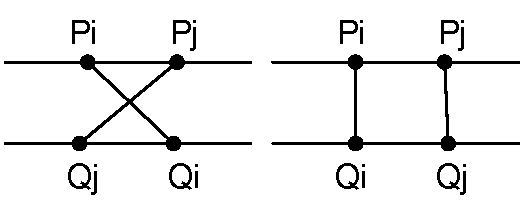
\includegraphics[width=0.25\textwidth]{pb2}
  \caption{Two-node cases of inversion vs intersection}
  \label{fig:pb2}
  \end{figure}

  Summarizing the two cases, we have the number of intersections $ = $ number of inversions for each pair $(i,j)$, thus the theorem holds. 

  (b)

  Given the conclusion in 1, permutations do not cause the number of inversions to change, this algorithm uses one list as the standard, takes in the other list, and calculates its number of inversions when compared against the standard. The algorithm's given in alg. \ref{alg:number-of-inversions-mergesort}.
  
  \begin{algorithm}[h]
  \caption{Number of inversions for one list against a permutated standard}
  \label{alg:number-of-inversions-mergesort}
    \begin{algorithmic}[1]
    \Function{numberOfInversions}{array}
      \State $n \gets len(array)$
      \If {$n < 2$}
        \State \Return $0$
      \EndIf
      
      \State $l1 \gets numberOfInversions(array[0]..array[n/2])$
      \State $l2 \gets numberOfInversions(array[n/2+1]..array[n])$

      \State \Return $l1 + l2 + countInversions(array, array[0]..array[n/2], array[n/2+1]..array[n])$
    \EndFunction

    \Function{countInversions}{original,l1,l2}
      \State $inversions \gets 0$
      \State $n \gets len(l1)$
      \State $pos \gets 0$

      \While {$l1.hasNext() \vee l2.hasNext()$}
        \If {$l1.hasNext() = false$}
          \State $original[pos] \gets l2.next()$
        \ElsIf {$l2.hasNext() = false$}
          \State $original[pos] \gets l1.next()$
        \ElsIf {$l1.next() < l2.next()$}
          \State $original[pos] \gets l1.next()$
        \Else
          \State $original[pos] \gets l2.next()$
          \State $i \gets n - l2.next()'s \quad position \quad in \quad l1$
          \State $inversions \gets inversions + i$
        \EndIf
        
        \State $pos \gets pos + 1$
      \EndWhile

      \State \Return $inversions$
    \EndFunction

    \end{algorithmic}
  \end{algorithm}
  
  \textbf{Time complexity:} this algorithm adds a constant-time inversion count to a recursive merge sort, thus the complexity is $O(n\log n)$

  \textbf{Correctness:} 

\item[3]{Celebrity iterative}

  Given an incident matrix representation of the graph, the algorithm's given in alg. \ref{alg:celebrity-iterative}. The algorithm takes in an $n \times n$ incident matrix (whose \textit{len}, number of persons, is $n$; and $matrix[i][j] = 1$ means person $i$ knows person $j$), and returns the index of the celebrity if there's one, otherwise returns -1. Matrix with less than two persons is considered to not have celebrities.

  \begin{algorithm}[h]
  \caption{Celebrity iterative}
  \label{alg:celebrity-iterative}
    \begin{algorithmic}[1]
    \Function{hasCelebrity}{matrix}
      \State $l \gets len(matrix)$
      \If $l < 2$
        \Return $-1$
      \EndIf
      \State $i \gets 0$
      \State $j \gets 1$

      \While $max(i, j) \leq l$
        \If {$matrix[i][j] = 1 \wedge matrix[j][i] = 0$}
          \State $i \gets max(i,j) + 1$
        \ElsIf {$matrix[j][i] = 1 \wedge matrix[i][j] = 0$}
          \State $j \gets max(i,j) + 1$
        \Else
          \State $i \gets max(i,j) + 1$
          \State $j \gets max(i,j) + 1$
        \EndIf
      \EndWhile

      \If {$i > l$}
        \State \Return $isCelebrity(matrix, j)$
      \Else
        \State \Return $isCelebrity(matrix, i)$
      \EndIf
    \EndFunction

    \Function{isCelebrity}{matrix, i}
      \For {person $p$ in matrix, $p \neq i$}
        \If {$matrix[p][i] = 0 \vee matrix[i][p] = 1$}
          \State \Return $-1$
        \EndIf
      \EndFor
      \State \Return $i$
    \EndFunction
    \end{algorithmic}
  \end{algorithm}

  \textbf{Time complexity:} this algorithm is $O(n)$, where $n$ is the number of persons.

  \textbf{Correctness:}

\item[4]{Diameter of tree}
  
  (a)

  Define the \textbf{height} of a rooted directed tree as the number of edges on the longest path from the root to a leaf. Algorithm is given in Alg \ref{alg:tree-diameter-recursive}.

  \begin{algorithm}[h]
  \caption{Diameter of a rooted directed tree's underlying undirected tree, recursive}
  \label{alg:tree-diameter-recursive}
    \begin{algorithmic}[1]
    \Function{findHeightOrDiameter}{root, findHeight, prevRoot}
      \If {$degree(root) = 1$}
        \State \Return $0$
      \EndIf
      \State $heights \gets []$
      \For {\textbf{each} $\{ n | n \in V, (n, root) \in E, n \neq prevRoot\}$}
        \State $heights.push(1 + findHeightOrDiameter(n, true, root))$
      \EndFor
      \If {$findHeight$}
        \State \Return $max(heights)$
      \Else
        \State \Return $max(heights) + 2^{nd}highest(heights)$
      \EndIf
    \EndFunction
    \end{algorithmic}
  \end{algorithm}

  This recursive algorithm takes in the root of a tree and produces the height of the tree, by each time removing the root and finding the maximum height among all resulting sub trees. The diameter of the tree would be the sum of the heights of two highest subtrees. Initial call to the algorithm should look like $findHeightOrDiameter(root, false, nil)$. This algorithm is $O(n)$, where $n$ is the number of nodes in the tree, because each node in the tree will be visited exactly once.

  (b)

  The iterative version of the algorithm is given in Alg \ref{alg:tree-diameter-iterative}.

  \begin{algorithm}[h]
  \caption{Diameter of a rooted directed tree's underlying undirected tree, iterative}
  \label{alg:tree-diameter-iterative}
    \begin{algorithmic}[1]
    \Function{findHeightOrDiameter}{root}
      \State $queue \gets [root]$
      \State $height0 \gets 0$
      \State $height1 \gets 0$
      \While {True}
        \State $nodeCount \gets queue.size()$
        \If {$nodeCount = 0$}
          \State \Return $height0 + height1$
        \EndIf
        \State $height \gets height + 1$
        \While {$nodeCount > 0$}
          \State $r \gets queue.dequeue()$
          \State $r.visited \gets true$
          \If {$degree(r)=1$}
            \If {$height > height0$}
              \State $height1 \gets height0$
              \State $height0 \gets height$
            \ElsIf {$height > height1$}
              \State $height1 \gets height$
            \EndIf
          \Else
            \For {\textbf{each} $ \{n | n \in V, (n, r) \in E, n.visited = false\}$}
              \State $queue.enqueue(n)$
            \EndFor
          \EndIf
          \State $nodeCount \gets nodeCount - 1$
        \EndWhile
      \EndWhile
    \EndFunction
    \end{algorithmic}
  \end{algorithm}

  This algorithm is $O(n)$, where $n$ is the number of nodes in the tree, because each node in the tree will be visited exactly once.

\end{description}

\end{document}
